\chapter{Lecture 13 - 3D data representation}

3D data is used across a vast array of fields, including cultural heritage, medicine, architecture, and security. It highlights that 3D models are no longer just for animation or gaming; they are critical for digital fabrication, archaeology, and eHealth. \par
There are four primary ways that 3D models are created:
\begin{itemize}[noitemsep]
    \item \textit{Manual modeling}: using dedicated SW like Blender
    \item \textit{Simulation}: generating models through computational physics or biological data
    \item \textit{Acquisition techniques}: using laser scanning or photogrammetry to digitize real-world objects. These techniques has overcome the modeling bottleneck, making 3D creation easier and less expensive.
    \item \textit{Generative AI}: emerging perspectives allow for image-to-3D or text-to-3D generation
\end{itemize}    

Once a model is acquired or created, it enters the \textbf{Geometry Processing} phase. This discipline is concerned with the mathematical models used to represent geometric data and the algorithms used to analyze, manipulate, and smooth that data to remove noise or reduce complexity.

\section{Surface representation}
\begin{definition}[Surface]
    In computer graphics, a surface is intuitively defined as a \emph{2D region within a 3D space} that has length and breadth but no thickness. If the surface is closed, it acts as the boundary of a 3D volume.
\end{definition}

There are two primary mathematical ways to define a surface analytically:
\begin{itemize}[noitemsep]
    \item Implicit surface is defined by an equation \(f(x, y, z) = 0\). As an example, the surface of a sphere, which is defined as \(x^2 + y^2 + z^2 - r^2 = 0\)
    \item Parametric surface is defined by a function mapping a 2D domain into 3D space. This uses coordinates (u, v) to determine the (x, y, z) position of every point on the surface.
\end{itemize}

While the analytical models are precise, they are \textit{difficult to apply to complex, real-world objects}. Consequently, computer graphics relies on discrete representations, which treat complex shapes as collections of simple "building blocks" glued together. The four most common blocks are \textbf{voxels, points, triangles, and quads}.

\subsubsection{Voxels - Volumetric representation}
This method considers a surface as the boundary of a solid volumetric object. It defines an \textbf{indicator function} that maps the 3D domain into a discrete binary domain where \textit{1 means solid and 0 means void}. \par
Alternatively, \textbf{signed distance fields} are a more advanced version that store the distance to the nearest surface at every point in a voxel grid. This provides more information than a simple occupancy map but requires more storage.\par
These are frequently used for massive 3D models, medical data (MRI/CT scans), and physics simulations.\par
This representation is excellent in tasks like rendering applications or volumetric field processing. They break down an object into regular structures for ease of use, but it can potentially occupy massive storage.

\begin{figure}[htbp]
    \centering
    
    \begin{subfigure}[b]{0.45\textwidth}
        \centering
        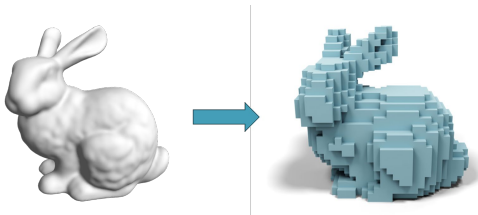
\includegraphics[width=0.6\linewidth]{imgs/lecture13/13.1 voxel representation.png}
        \caption{}
        \label{fig:13.1a}
    \end{subfigure}
    \hfill
    \begin{subfigure}[b]{0.45\textwidth}
        \centering
        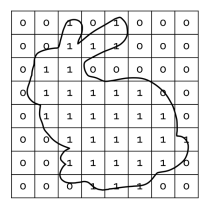
\includegraphics[width=0.4\linewidth]{imgs/lecture13/13.2 voxel representation.png}
        \caption{}
        \label{fig:13.1b}
    \end{subfigure}

    \caption{Voxel representation}
    \label{fig:13.1}
\end{figure}

\subsubsection{Point clouds}
Point clouds are unordered collections of point samples often originating from 3D scans. They are compact, easy to handle, and excellent for fast rendering of massive datasets or real-time tasks like autonomous driving. But, because they are just a collection of points, they are often irregular and do not truly represent a continuous surface.

\begin{figure}[htbp]
    \centering
    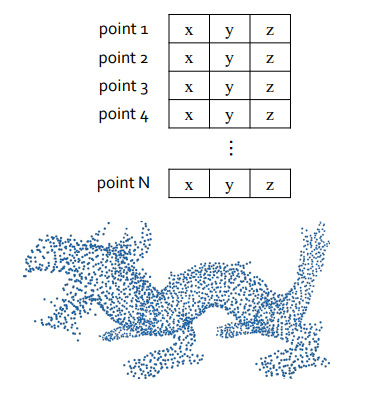
\includegraphics[width=0.4\linewidth]{imgs/lecture13/13.3 point cloud.png}
    \caption{Point cloud}
    \label{fig:13.2}
\end{figure}

\subsubsection{Triangle mesh}
The triangle meshes are the de facto standard for geometry processing. They represent a surface as a collection of triangles, which offers several advantages (Planarity and convexity, approximation power and so on). Every triangle is inherently flat and simple to calculate. \par
They are the most efficient way to store generic 3D surfaces for movies, video games, and 3D modeling. Unlike regular voxel grids, meshes can adapt their density, using many small triangles for detailed areas and fewer large ones for flat surfaces.

\section{Topological foundations}
To process geometric data accurately, computer graphics relies on topology to describe how elements are connected, regardless of their specific shape or position.

\begin{definition}[Simplice]
    The most basic building block used to construct a complex 3D shape is called a \emph{simplex}. A k-simplex is mathematically defined as the convex hull of h+1 affinely independent points, called vertices.
\end{definition}

There are four possible types of simplices: 0-simplex (a single point, a vertex); 1-simplex (a line segment connecting two points); 2-simplex (a triangle defined by three points); 4-simplex (a tetrahedron, a 3D pyramid shape defined by four points).

\begin{figure}
    \centering
    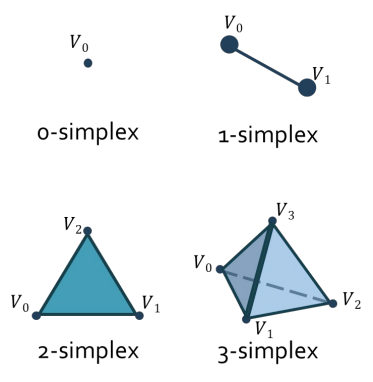
\includegraphics[width=0.35\linewidth]{imgs/lecture13/13.4 simplices.png}
    \caption{Simplices}
    \label{fig:13.3}
\end{figure}

\subsubsection{Faces and orientation}

\begin{definition}[Proper face]
    A proper face of a k-simplex (a simplex with k dimensions) is another simplex whose set of vertices is a non-empty proper subset of the vertices of the original simplex.
\end{definition}

In simpler terms, if you take some, but not all, of the points that define a shape and use them to form a new, lower-dimensional shape, that new shape is a proper face. For example, A 1-simplex (a line)'s proper faces are its two vertices (0-simplices); a 2-simplex(a triangle)'s proper faces are its three edges (1-simplices) and 3 vertices (0-simplices)

\subsubsection{Simplicial complexes}
A simplicial complex is a structured obtained by "gluing" the simplices. To be considered a proper complex, the collection must follow two rules:

\begin{itemize}[noitemsep]
    \item Any two simplices in the collection can only meet along a common face
    \item If a simplex is in the collection, all of its faces must also be included in the collection. 
\end{itemize}

The \textbf{dimension} of the simplicial complex is the maximum dimension of its simplices. A k-dimensional simplicial complex is homogeneous if it is made of k-simplices and their faces.

\begin{definition}[Homogeneity]
    A simplicial complex is called homogeneous if all its primary components are of the same dimension and do not have any dangling parts of lower dimension
\end{definition}

Under the definition of homogeneity, a triangle mesh is a homogeneous 2D simplicial complex because it is composed entirely of triangles and their shared edges and vertices.

\section{Topological relations}

\begin{definition}[Adjacency and incidency]
    Two k-simplices A and B are \emph{m-adjacent} (m<k) if there exists an m-simplex which is a proper face of both A and B (A and B share a common face).\par
    Two simplices are \emph{incident} if one is a proper face of the other
\end{definition}

For example, two triangles (2-simplices) sharing an edge (1-simplex) are 1-adjacent;  two triangles sharing a vertex (0-simplex) are 0-adjacent.\par
Two vertices (0-simplices) are adjacent if they are incident to a common edge (1-simplex).

\begin{definition}[Boundary]
    For a triangle mesh, the boundary is defined as the union of all edges that are incident to exactly one face. In a closed object with no holes, there is no boundary.
\end{definition}

\subsubsection{Manifoldness - Well-behaved surfaces}
Computer graphics often assumes surfaces are 2D manifolds, which is a way of saying they behave like physical, non-degenerate solids with no infinitely thin parts.\par
A continuous definition says that a surface is a manifold is every point on it has a neighborhood that can be continuously deformed into a disk.

\begin{figure}
    \centering
    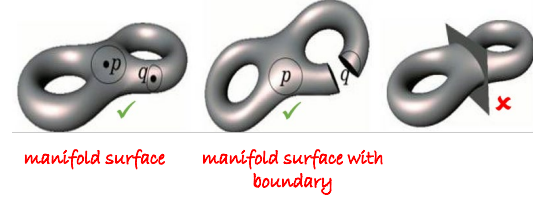
\includegraphics[width=0.5\linewidth]{imgs/lecture13/13.5 manifold.png}
    \caption{Manifoldness}
    \label{fig:13.4}
\end{figure}

On discrete rules for triangle meshes to be considered manifold, it must follow two specific rules:
\begin{itemize}[noitemsep]
    \item \textbf{Vertex rule}: the "star" (the collection of triangles surrounding a vertex) must form a single connected "fan". You must be able to travel between any two triangles in the star without leaving the neighborhood 
    \item \textbf{Edge rule}: every edge must be incident to at least two faces(one for a boundary, two for an interior).
\end{itemize}

\begin{figure}
    \centering
    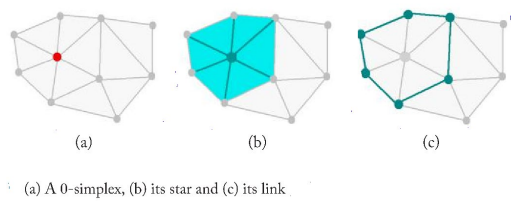
\includegraphics[width=0.5\linewidth]{imgs/lecture13/13.6 star and link.png}
    \caption{Star and link}
    \label{fig:13.5}
\end{figure}

In the fig.\ref{fig:13.5}, the simplex in question is a vertex (0-simplex), and its "\textbf{star}" is the union of all the simplices containing the said vertex forming the figure b. Its \textbf{link} is all the faces of the simplices in the star of the vertex that do not intersect with it. 

\subsection{Normals on meshes}
Normals (vectors perpendicular to the surface) are critical for tasks like shading.\par
In a continuous mathematical model, the unit surface normal vector at a specific point p is the vector that is orthogonal to the tangent plane at that point. This tangent plane is spanned by the tangent vectors to curves passing through p, and is calculated using the partial derivatives of a regular surface parametrization.\par
In the discrete case, because triangle meshes are discrete collections of flat faces, evaluating normals requires a different approach. Because the triangles are perfectly flat (planar), their normals are constant and easily calculated using the cross product of two edges. \par
To get a smooth look across a jagged mesh (such as in Gouraud or Phong shading), normals must be evaluated at the vertices. The standard is to compute the vertex normal as a weighted average of the normals of all triangles in its star. Using constant weights can be counterintuitive on irregular meshes, so weighting by triangle area or angle is preferred for better results. 